\chapter{Conception}
In order to do a proper conception of the bandwidth limiter for \acs{SCIONLab}, we have to formalize the requirements. We want to achieve the following:

\begin{enumerate}
\item[$\bullet$]The \acs{SCIONLab} administrators should be able to set a maximal bandwidth that is available to the user-\acsp{AS}.
\item[$\bullet$]The administrators of the user-\acsp{AS} (the customers) should be able to set an upper limit for the bandwidth in the range of $[0,x]$ where $x$ is the bandwidth limit set by the \acs{SCIONLab} administrators.
\item[$\bullet$] The above mentioned limits should be enforced automatically by only making configurations on the \acsp{AP}.
\end{enumerate}

We split up these three requirements into two sections. The first two belong to the front end of the project, where as the third requirement is part of the back end.

\section{Front end}

The front end part of the project is all about the \acs{SCIONLab} server. The implementation of that server can be found on \href{https://github.com/netsec-ethz/scionlab}{github.com}. There is already a configuration page, where the customers can set the desired configuration for their user-\acs{AS}. On the same configuration page we simply add a field, where the customers can insert a bandwidth limit between 0 and the limit set by the \acs{SCIONLab} administrators. Other bandwidth limits get already rejected by the form.
\\
The \acs{SCIONLab} server stores information about the entire topology of the \acs{SCIONLab} network, including the links from the \acsp{AP} to the user-\acsp{AS}. Per link there is a field that stores the maximal bandwidth for that link. This field exists but is currently not used. Therefore we simply set that attribute to the bandwidth limit that the customer chose.
\\
The \acs{SCIONLab} server regularly generates files according to its data model that are then sent to the \acsp{AP}, in order to configure them for newly added or updated user-\acsp{AS}. These files are packed in a tarball and then delivered and unpacked on the \acsp{AP}. We can use this mechanism to deliver the information we need, in order to enforce the bandwidth limitations, to the \acsp{AP}. So we simply add a \ac{JSON}-file called \textit{link\_info.json} to that tarball, which holds the information we need to perform bandwidth limitations.

\section{Back end}

\begin{figure}[h]
	\centering
	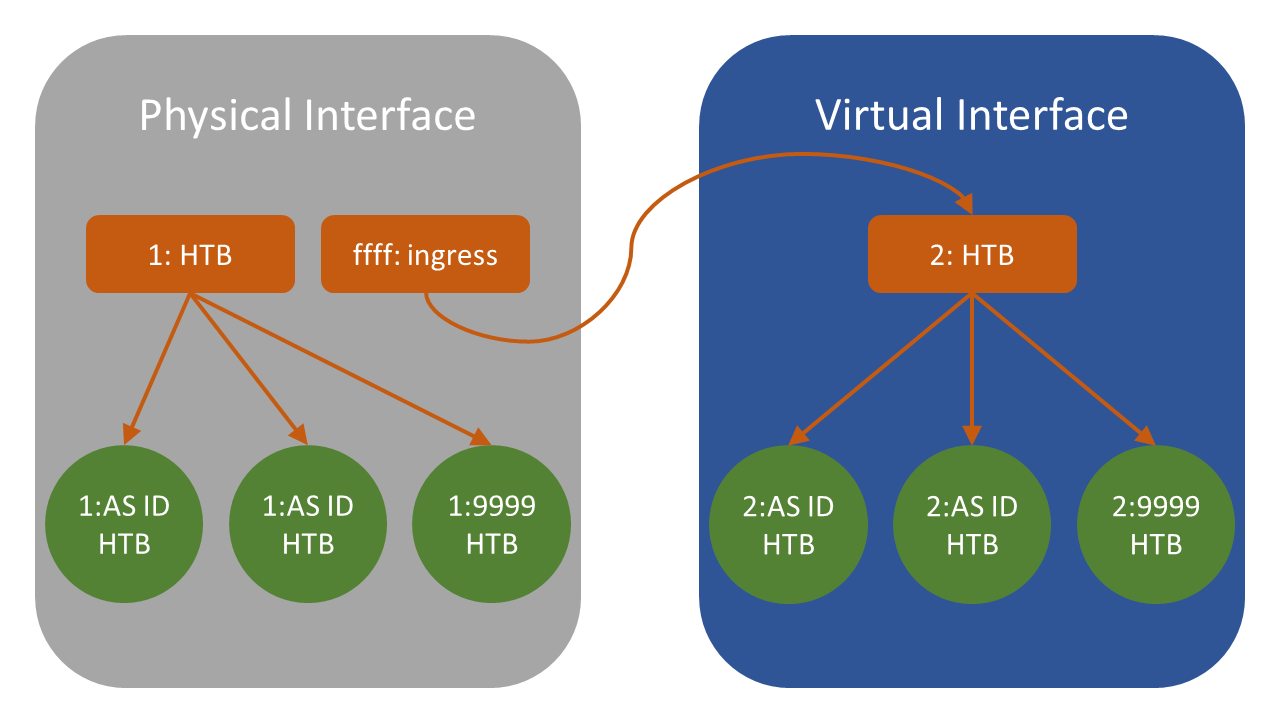
\includegraphics[width=\textwidth]{img/QDISC-Set-up.png}
	\caption{QDISC/Class hierarchy}
	\label{QDISC-Set-up}
\end{figure}